\appendix
\section{Proof of Lower Bound}

This appendix completes the proof of the bound in the text that
\begin{align}
-\int p_0(z) \log p_\theta(z) 
& \leq \KL{q_\gamma(x|z) p_0(z)}{p_\theta(z|x)p(x)}
 - \Exp{\log p_0(z)}\label{eq:appendix1} 
\end{align}
where $p_0$ is the standard normal density, and $p_\theta(z) = \int p_\theta(z|x) p(x) \,dx$.
As described in the text, introducing a a variational distribution $q_\gamma (x|z)$ yields
\begin{equation}
-\int p_0(z) \log p_\theta(z) \,dz \leq -\iint p_0(z) q_\gamma(x|z) \log \frac{p_\theta(z|x)p(x)}{q_\gamma(x|z)} \,dx \,dz.\label{eq:jensen}
\end{equation}
Starting from \eqref{eq:jensen}, we obtain a new upper bound by adding a trivial KL divergence to the right hand side of the above inequality
\begin{align}
-\int p_0(z) \log p_\theta(z) \,dz
  &\leq -\iint p_0(z) q_\gamma(x|z) \log \frac{p_\theta(z|x)p(x)}{q_\gamma(x|z)} \,dx \,dz \nonumber\\
  &= \iint p_0(z) q_\gamma(x|z) \log \frac{q_\gamma(x|z)}{p_\theta(z|x)p(x)} \,dx \,dz + \int p_0(z) \log \frac{p_0(z)}{p_0(z)} \,dz \label{eq:top-ineq}
\end{align}
Now for the upper term in the KL, we have that
\begin{align*}
	\int p_0(z) \log {p_0(z)} \,dz = \int p_0(z) \log {p_0(z)} \left(\int q_\gamma(x|z) \,dx \right)\,dz 
	 = \iint p_0(z) q_\gamma(x|z) \log {p_0(z)} \,dx \,dz.
\end{align*}
Combining with \eqref{eq:top-ineq} yields
\begin{align} 
H(Z, F_\theta(X)) &\leq \iint p_0(z) q_\gamma(x|z) \log \frac{q_\gamma(x|z)}{p_\theta(z|x)p(x)} \,dx \,dz
        + \iint p_0(z) q_\gamma(x|z) \log {p_0(z)} \,dx \,dz \nonumber\\
        & \qquad\quad - \int p_0(z) \log p_0(z) \,dz \nonumber\\
        &= \iint p_0(z) q_\gamma(x|z) \log \frac{q_\gamma(x|z) p_0(z)}
        {p_\theta(z|x)p(x)} \,dx \,dz
    - \int p_0(z) \log p_0(z) \,dz \nonumber\\
    &=  \KL{q_\gamma(x|z) p_0(z)}{p_\theta(z|x)p(x)} - \int p_0(z) \log p_0(z) \,dz, \nonumber
\end{align}	
% Since the loss function $d$ is nonnegative, we further have
% \begin{equation*}
% 0 \leq \int p_0(z) d(z, F_\theta(G_\gamma(z))) \,dz = \iint p_0(z)q_\gamma(x | z) d(z, F_\theta(x)) \,dx \,dz = \Exp{d(z, F_\theta(x))}
% \end{equation*}
% so that
% \begin{align} 
% H(Z, F_\theta(X)) &\leq \KL{q_\gamma(x|z) p_0(z)}{p_\theta(z|x)p(x)} - \int p_0(z) \log p_0(z) \,dz + \Exp{d(z, F_\theta(x))}\nonumber\\
%         &:= \calO(\gamma, \theta), 
% \end{align}
which completes the proof.



\section{Proof of Proposition 1}
\begin{proposition}
Suppose that there exist parameters $\theta^*, \gamma^*$ such that 
$\calO(\gamma^*, \theta^*)= H[p_0],$ where $H$ denotes Shannon entropy. Then $(\gamma^*, \theta^*)$ minimizes $\calO$, and we further have that
\begin{align*}
 p_{\theta^*}(z) &:= \int p_{\theta^*}(z|x) p(x) \,dx = p_0(z) \\
q_{\gamma^*}(x) &:= \int q_{\gamma^*}(x|z) p_0(z) \,dz = p(x).
\end{align*}
\end{proposition}

\begin{proof}
From information theory, we know that
$ \KL{q_\gamma(x|z) p_0(z)}{p_\theta(z|x)p(x)} \geq 0.$
Additionally, we have that $\Exp{d(z, F_\theta(x))} \geq 0,$. Moreover, by definition of $\Exp{}$ in the proposition,
\begin{align*}
-\Exp{\log p_0(z)}&= -\iint p_0(z) q_\gamma(x|z) \log p_0(z) \,dz dx = -\int p_0(z) \log p_0(z) \,dz  \int q_\gamma(x|z) \, dx \\
&= -\int p_0(z) \log p_0(z) \,dz,
\end{align*}
which is the definition of the Shannon entropy $H[p_0]$ of $p_0$.

This implies that
\begin{align*}
\calO(\gamma, \theta) &=  \KL{q_\gamma(x|z) p_0(z)}{p_\theta(z|x)p(x)}
 - \Exp{\log p_0(z)}
+ \Exp{d(z, F_\theta(x))} \\
&\geq - \Exp{\log p_0(z)} \\ &= H[p_0].
\end{align*}
This bound is attained with equality when $q_\gamma(x|z) p_0(z) = p_\theta(z|x)p(x)$,
and when $F_\theta$ inverts $G_\gamma$ on the data distribution, i.e.,
when  $F_\theta(G_\gamma(z)) = z$
for all $z$. (Note that this
statement does not require
$G$ to be invertible outside
of its range.)

Now, if $\calO(\gamma^*, \theta^*) = H[p_0],$ subtracting the entropy
from both sides implies that
$\KL{q_\gamma(x|z) p_0(z)}{p_\theta(z|x)p(x)} = 0.$
Because the optimum of the KL divergence  is unique, we then have that  $q_{\gamma^*}(x|z) p_0(z) = p_{\theta^*}(z|x)p(x).$

Integrating both sides over $x$ yields the first equality in the proposition,
and integrating over $z$ yields the second.
\end{proof}

\section{Discriminator Architecture for ALI and \acronym}
When using ALI and VEEGAN, the original DCGAN discriminator needs to be augmented in order allow it to operate on pairs of images and noise vectors.
In order to achieve this, we flatten the final convolutional layer of DCGAN's discriminator and concatenate it with the input noise vector. Afterwards, we run the concatenation through a hidden layer, and then compute $D_\omega(z,x)$ through a linear transformation.

\begin{table}[h]
\centering
\caption{ALI and \acronym Discriminator Architecture.}
\label{tab:arch}
\begin{tabular}{|c|c|c|c|}
\hline
\multicolumn{1}{|l|}{\textbf{Operation}} & \textbf{\#Output} & \multicolumn{1}{l|}{\textbf{BN?}} & \multicolumn{1}{l|}{\textbf{Activation}} \\ \hline
{$D_\omega(x)$}                            & \multicolumn{3}{l|}{}                                                                            \\ \hline
Conv                                     & 64                & False                             & Leaky ReLU                               \\ \hline
Conv                                     & 128               & True                              & Leaky ReLU                               \\ \hline
Conv                                     & 256               & True                              & Leaky ReLU                               \\ \hline
Conv                                     & 512               & True                              & Leaky ReLU                               \\ \hline
Flatten                                  & -                 & -                                 & -                                        \\ \hline
\textbf{$\sigma(D_\omega(z,x))$}                          & \multicolumn{3}{l|}{Concatenate $D_\omega(x)$ and $z$ along the first axis.}                      \\ \hline
Fully Connected                          & 512               & False                             & Leaky ReLU                               \\ \hline
Fully Connected                          & 1                 & False                             & Sigmoid                                  \\ \hline
\end{tabular}
\end{table}

\section{Inference}
While not the focus of this work, our method can also be used for inference as in the case of ALI and BiGAN models. Figure \ref{fig:ali_inf} shows an example of inference on MNIST. The top row samples are from the dataset. We extract the latent representation vector for each of the real images by running them through the trained reconstructor and then use the resulting vector in the generator to get the generated samples shown in the bottom row of the figure.
\begin{figure}
  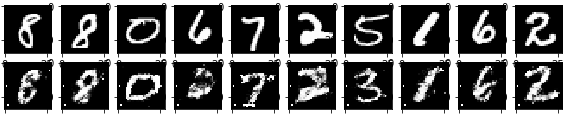
\includegraphics[width=\linewidth]{pics/ali_inference.png}
  \caption{\acronym method can be used like ALI to perform inference. The means output from the reconstructor network for the real images in the top row are used as the latent features to samples the generated images in the bottom row. \AS{Either include reconstructions for other methods, or cut this figure entirely.
  What does this demonstrate that the other figures do not?}}
  \label{fig:ali_inf}
\end{figure}

\section{Adversarial Methods for Autoencoders}
In order to quantify contrast the effect of autoencoding of noise in \acronym with autoencoding of data in DAE methods \citep{Che2017ModeRG,larsen2015autoencoding} we train DAE version of \acronym by simply using the reconstructor network as an inference network. As mentioned before, careful tuning of the weighing parameter $\lambda$ is needed to ensure that the $\ell_2$ loss is only working as a regularizer. Therefore, we run a parameter sweep for $\lambda$. As shown in figure \ref{fig:dae_cifar} we were not able to obtain any meaningful images for any of the tested values.   
\AS{We need a sentence or two saying why we do this}

\AS{Suggest we cut Figure 7; I cannot see how it provides
evidence for any proposition. Also, "without $\calO$"
is unclear; is this just $\lambda = 0$?}

\AS{Capture in Figure 8: Are you sure the l2 loss is dominating
or are you guessing from the images? If the latter, I would cut 
this. We don't want to speculate without being very
clear that is what we are doing. And here, it's unnecessary
to speculate. Just say the images are bad.}

% \begin{figure}[!htb]
% \caption{Density plots for GANs with data Autoencoders on 2D Grid dataset. We found that for even $\lambda=0.001$ the $ell_2$ term alone is able to capture all the eight modes. Therefore, it is hard to conclude the contribution of adversarial learning in the generative process in such methods that directly apply auxiliary loss to the data.}\label{fig:dae}
% \begin{subfigure}{0.18\textwidth}
%   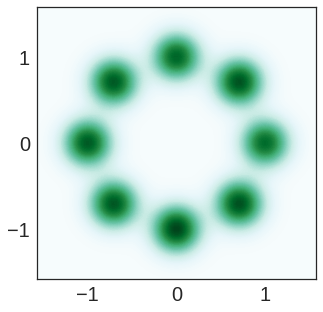
\includegraphics[width=\linewidth]{pics/true_ring.png}
%   \caption{True Data}\label{fig:true_grid}
% \end{subfigure} 
% \begin{subfigure}{0.18\textwidth}
%   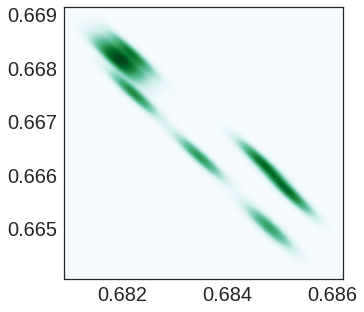
\includegraphics[width=\linewidth]{pics/gan_ring.png}
%   \caption{$\lambda=0$}\label{fig:gan_grid}
% \end{subfigure}
% \begin{subfigure}{0.18\textwidth}
%   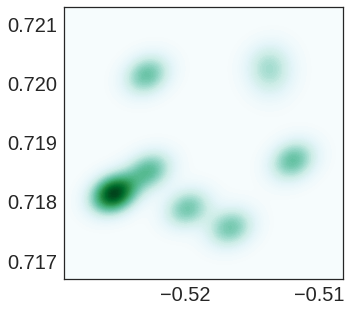
\includegraphics[width=\linewidth]{pics/001.png}
%   \caption{$\lambda=0.001$}\label{fig:10_ring}
% \end{subfigure}
% \begin{subfigure}{0.18\textwidth}
%   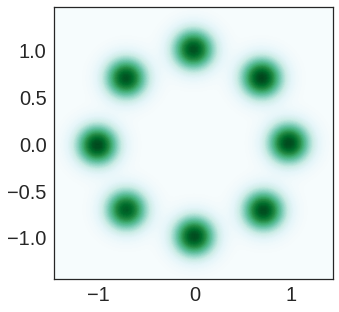
\includegraphics[width=\linewidth]{pics/100.png}
%   \caption{$\lambda=0.005$}\label{fig:100_ring}
% \end{subfigure}
% \begin{subfigure}{0.18\textwidth}%
%   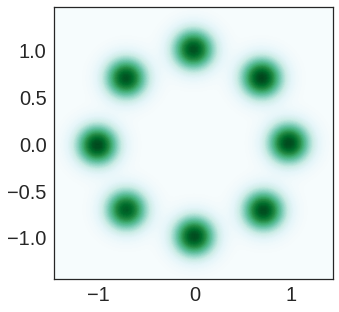
\includegraphics[width=\linewidth]{pics/100.png}
%   \caption{Without $\hat{\calO}$}\label{fig:100_ring}
% \end{subfigure}
% \end{figure}

\begin{figure}[!htb]
\caption{CIFAR 10 samples from GANs with data Autoencoders. We did a parameter sweep over the value of $\lambda$ but were unable to generate any meaningful images for any of the values. Figure \ref{fig:ng} is generated entirely from the $\ell_2$ loss.}\label{fig:dae_cifar}
\begin{subfigure}{0.24\textwidth}
  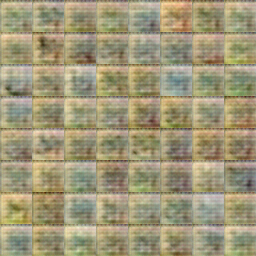
\includegraphics[width=\linewidth]{pics/l_007.png}
  \caption{$\lambda=0.007$}\label{fig:7}
\end{subfigure} \hfill
\begin{subfigure}{0.24\textwidth}
  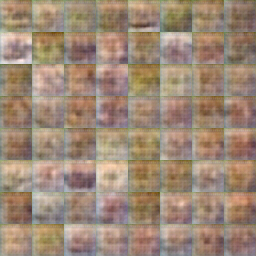
\includegraphics[width=\linewidth]{pics/l_001.png}
  \caption{$\lambda=0.01$}\label{fig:1}
\end{subfigure} \hfill
\begin{subfigure}{0.24\textwidth}
  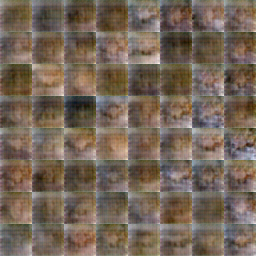
\includegraphics[width=\linewidth]{pics/l_005.png}
  \caption{$\lambda=0.05$}\label{fig:5}
\end{subfigure} \hfill
\begin{subfigure}{0.24\textwidth}
  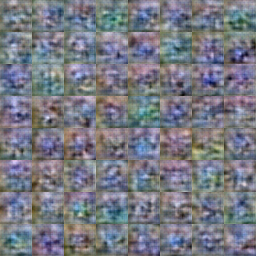
\includegraphics[width=\linewidth]{pics/ae_nogan.png}
  \caption{Only $\ell_2$}\label{fig:ng}
\end{subfigure}
\end{figure}


\section{Stacked MNIST Qualitative Results}
Qualitative results from the Stacked MNIST dataset for all the 4 methods.
\begin{figure}[!htb]
\caption{Samples from trained models for Stacked MNIST dataset.}\label{fig:sm}
\begin{subfigure}{0.18\textwidth}
  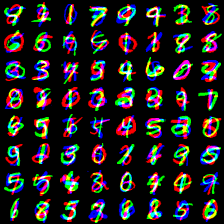
\includegraphics[width=\linewidth]{pics/true_sm.png}
  \caption{True Data}\label{fig:true_sm}
\end{subfigure} 
\begin{subfigure}{0.18\textwidth}
  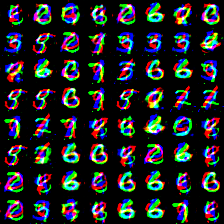
\includegraphics[width=\linewidth]{pics/dcgan_sm.png}
  \caption{DCGAN}\label{fig:gan_sm}
\end{subfigure}
\begin{subfigure}{0.18\textwidth}
  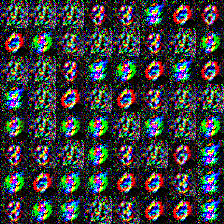
\includegraphics[width=\linewidth]{pics/ali_sm.png}
  \caption{ALI}\label{fig:ali_sm}
\end{subfigure}
\begin{subfigure}{0.18\textwidth}
  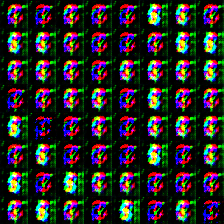
\includegraphics[width=\linewidth]{pics/unrolled_sm.png}
  \caption{Unrolled}\label{fig:unrolled_sm}
\end{subfigure}
\begin{subfigure}{0.18\textwidth}%
  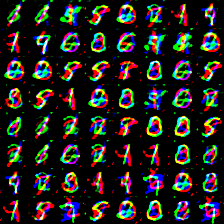
\includegraphics[width=\linewidth]{pics/veegan_sm.png}
  \caption{\acronym}\label{fig:veegan_sm}
\end{subfigure}
\end{figure}

\section{CelebA Random Sample from ALI and \acronym}

Additionally, we compared ALI and \acronym models  on the much bigger CelebA dataset \citep{liu2015faceattributes} of faces.
Our goal is to test how robust each method is when used without  extensive tuning of model architecture and hyperparameters
on a new dataset.
Therefore we use the same model architectures and hyperparameters
as we did on the CIFAR-10 data.
While ALI failed to produce any meaningful images, \acronym generates high quality images of faces. Please note that this does not mean that ALI fails on CelebA in general. Indeed, as \cite{ali2016} show, given higher capacity reconstructor and discriminator with the right  hyperparameters, it 
is possible to generate good quality images on this dataset. 
Rather, this experiment only suggests that for the simple network that we use for Stacked MNIST and CIFAR experiments, \acronym learning method was able to produce reasonable images without any further tuning or hyper parameter search.
\begin{figure}[H]
\centering
  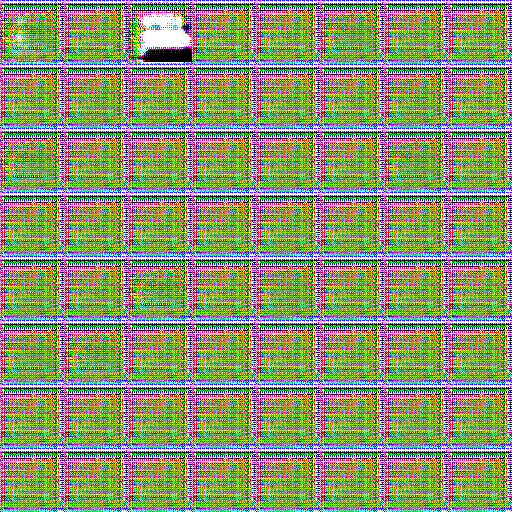
\includegraphics[width=.6\linewidth]{pics/ali_face.png}
  \caption{ALI on CelebA with simple DCGAN architecture
  and without tweaking of hyperparameters.}
  \label{fig:dcgan_cifar}
\end{figure}
\begin{figure}[H]
\centering
  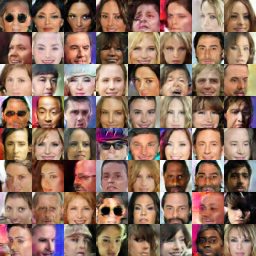
\includegraphics[width=.6\linewidth]{pics/veegan_face.png}
  \caption{\acronym on CelebA with simple DCGAN architecture
  and default hyperparameters.}
  \label{fig:ali_cifar}
\end{figure}


\section{CIFAR 10 Random Sample from \acronym}
% \begin{figure}[!htb]
% \caption{Inference as Optimization Metric Samples for CIFAR 10. In each of the two sub-figures, the first column comes from the dataset, followed by columns from DCGAN, ALI, Unrolled and \acronym respectively. }\label{fig:cifar}
% \begin{subfigure}{0.48\textwidth}
%   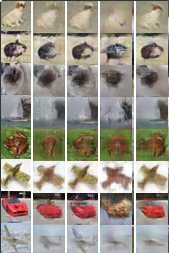
\includegraphics[width=\linewidth]{pics/cifar.png}
%   \caption{Sample 1}\label{fig:col1}
% \end{subfigure} \hfill
% \begin{subfigure}{0.48\textwidth}
%   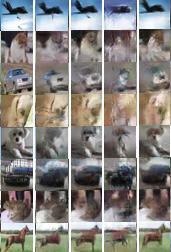
\includegraphics[width=\linewidth]{pics/cifar1.png}
%   \caption{Sample 2}\label{fig:col2}
% \end{subfigure}
% \end{figure}

Randomly generated samples for CIFAR 10 dataset for all the 4 methods.
\begin{figure}[H]
\centering
  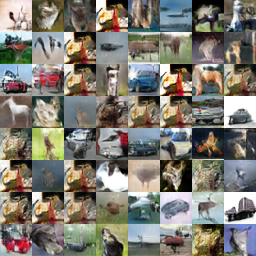
\includegraphics[width=.6\linewidth]{pics/dcgan_final.png}
  \caption{DCGAN on CIFAR 10 Dataset }
  \label{fig:dcgan_cifar}
\end{figure}
\begin{figure}[H]
\centering
  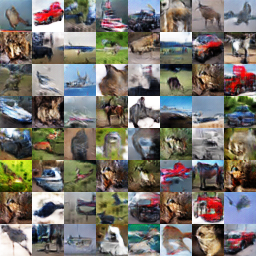
\includegraphics[width=.6\linewidth]{pics/ali_final.png}
  \caption{ALI on CIFAR 10 Dataset }
  \label{fig:ali_cifar}
\end{figure}
\begin{figure}[H]
\centering
  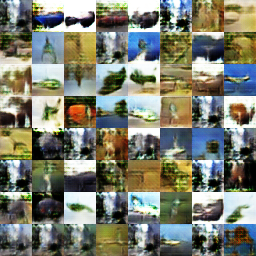
\includegraphics[width=.6\linewidth]{pics/unrolled_final.png}
  \caption{Unrolled GAN on CIFAR 10 Dataset }
  \label{fig:unrolled_cifar}
\end{figure}
% \begin{figure}[H]
%   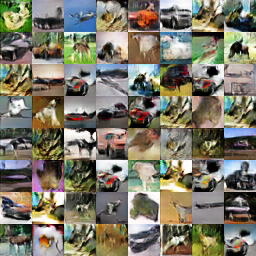
\includegraphics[width=.6\linewidth]{pics/cifar_final.png}
%   \caption{\acronym on CIFAR 10 Dataset }
%   \label{fig:veegan_cifar_}
% \end{figure}
\begin{figure}[H]
\centering
  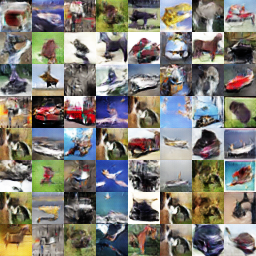
\includegraphics[width=.6\linewidth]{pics/veegan_cifar.png}
  \caption{\acronym on CIFAR 10 Dataset }
  \label{fig:veegan_cifar}
\end{figure}

